\documentclass[tikz,border=10pt]{standalone}
\usetikzlibrary{shapes.geometric, arrows.meta}

\tikzset{
    block/.style = {rectangle, draw, fill=blue!20, 
        text width=6em, text centered, rounded corners, minimum height=4em},
    line/.style = {draw, thick, -Stealth},
    cloud/.style = {draw, ellipse,fill=red!20, node distance=3cm,
        minimum height=7em}
}

\begin{document}
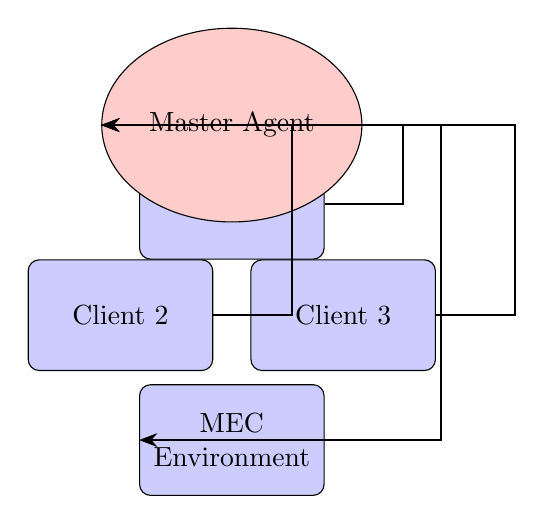
\begin{tikzpicture}[node distance=2cm]

\node (Client1) [block] {Client 1};
\node (Client2) [block, below left of=Client1] {Client 2};
\node (Client3) [block, below right of=Client1] {Client 3};

\node (MasterAgent) [cloud, above of=Client1, yshift=-2cm] {Master Agent};

\node (MEC) [block, below of=MasterAgent, yshift=-2cm] {MEC Environment};

% Drawing lines between nodes
\draw [line] (Client1.east) -- ++(1,0) |- (MasterAgent.west);
\draw [line] (Client2.east) -- ++(1,0) |- (MasterAgent.west);
\draw [line] (Client3.east) -- ++(1,0) |- (MasterAgent.west);

\draw [line] (MasterAgent.east) -- ++(1,0) |- (MEC.west);

\end{tikzpicture}
\end{document}